\section{Задание 2}

Дано два числа x, y и знак арифметической операции (+, -, *, /). Найти x+y, x-y, x*y, x/y, в зависимости от введённого знака. В случае ошибки в знаке или деления на 0 вывести сообщение об ошибке.

\begin{center} 
  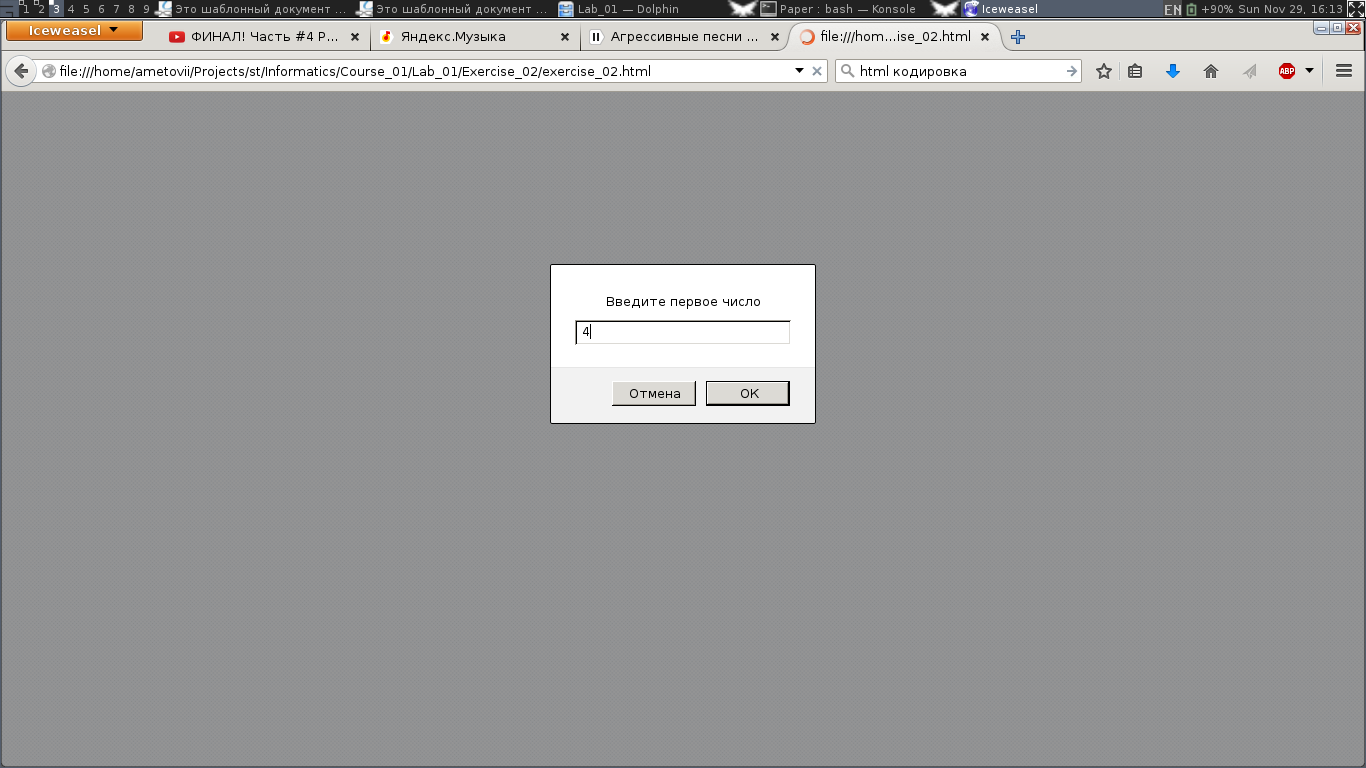
\includegraphics[width=15cm]{img/0201.png}
  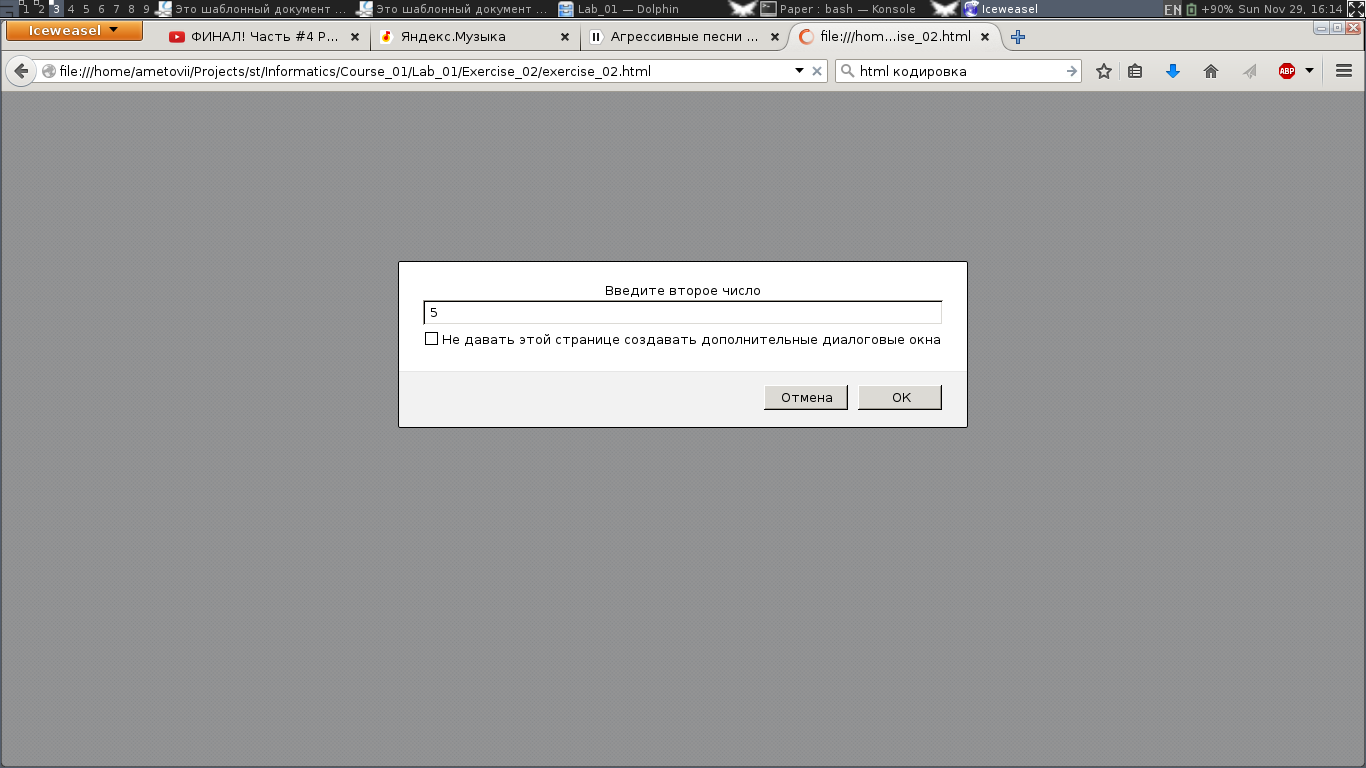
\includegraphics[width=15cm]{img/0202.png}
  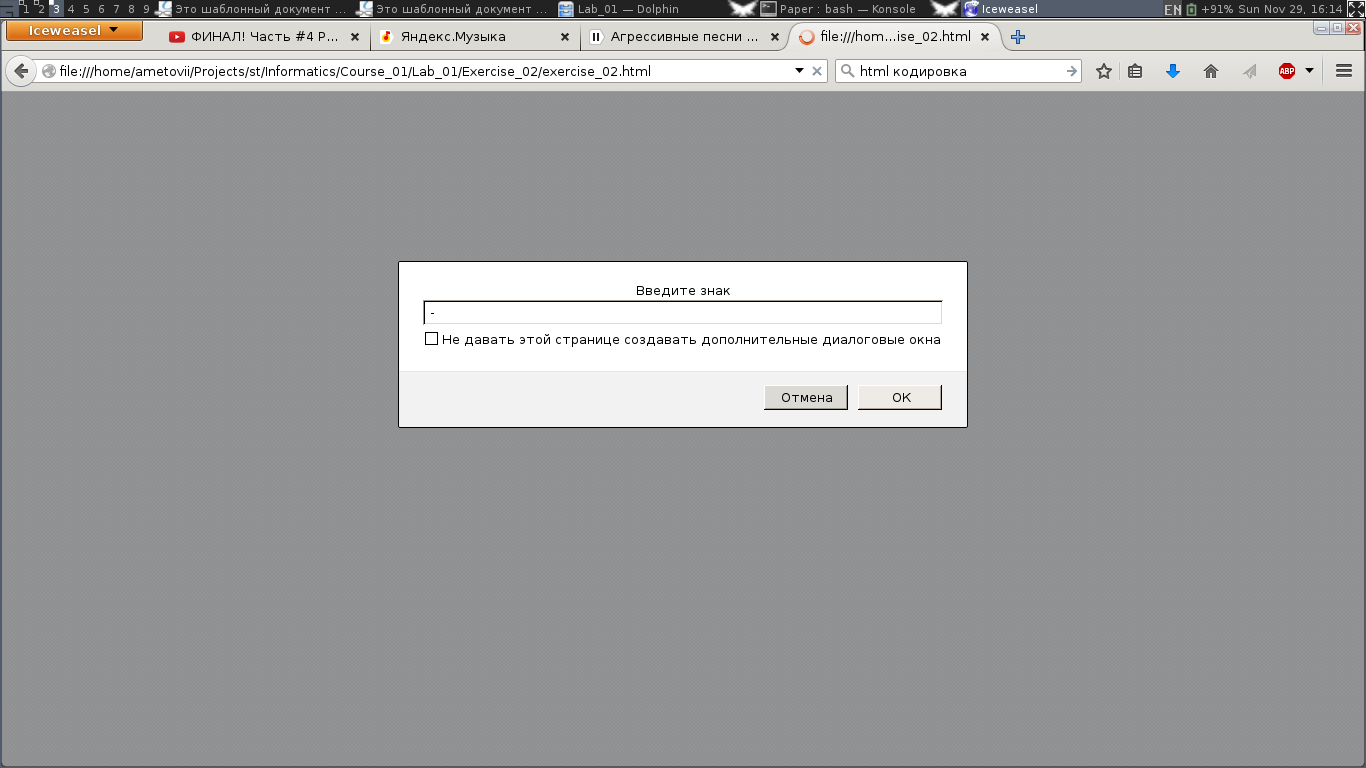
\includegraphics[width=15cm]{img/0203.png}
  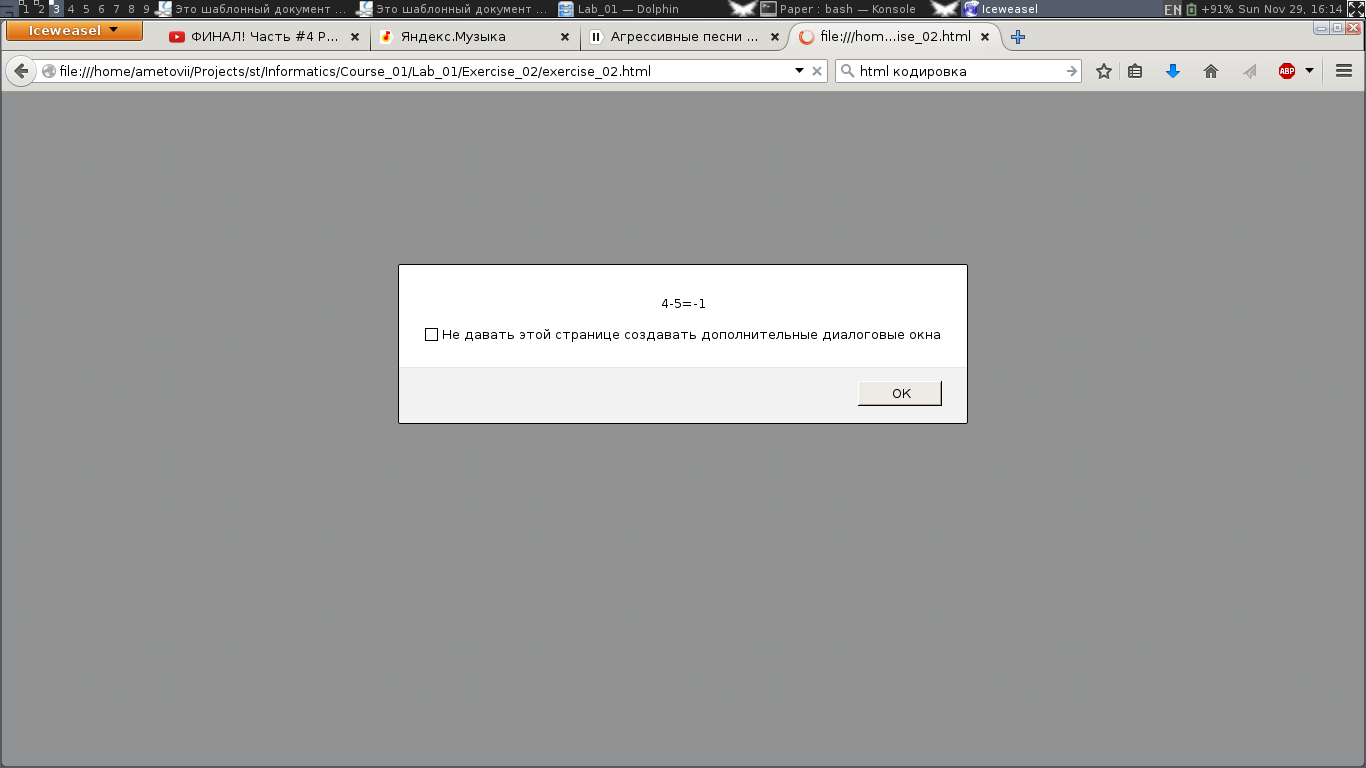
\includegraphics[width=15cm]{img/0204.png}
  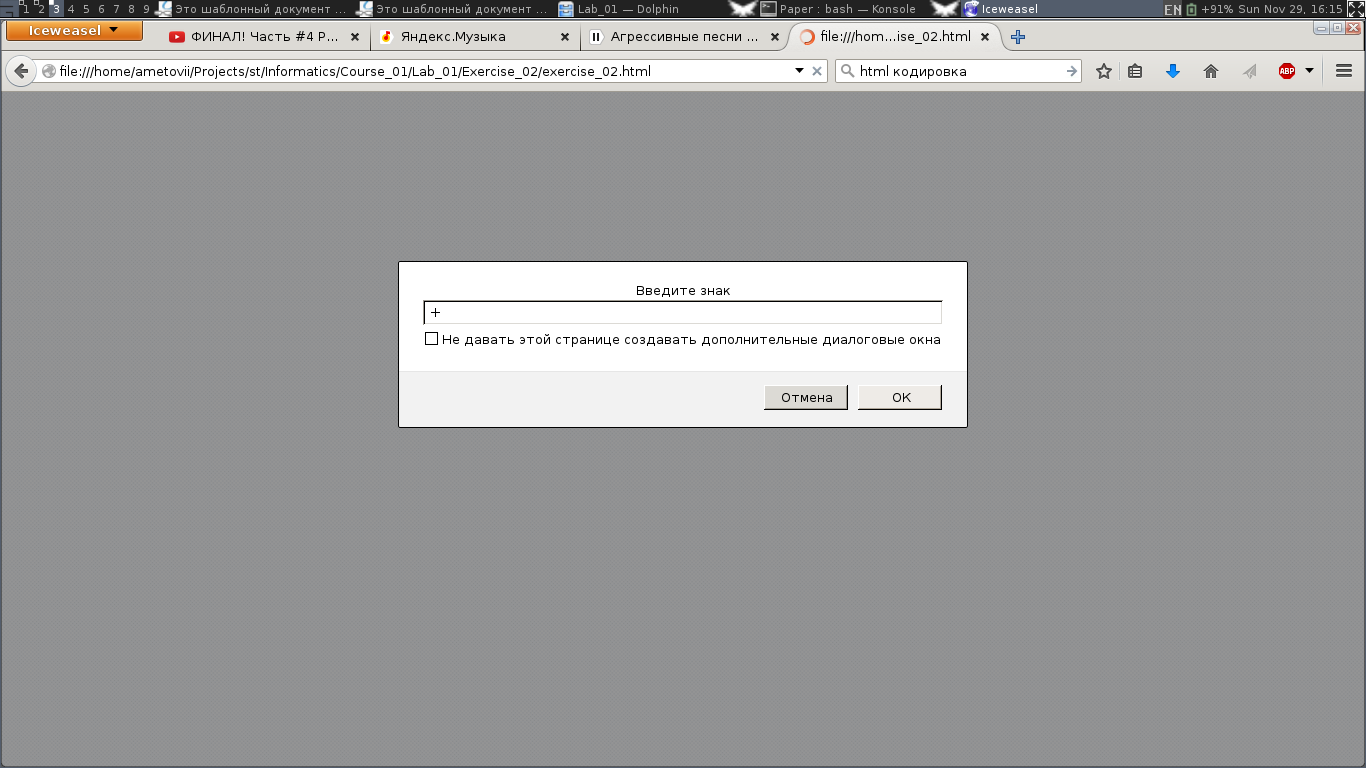
\includegraphics[width=15cm]{img/0205.png}
  
\includegraphics[width=15cm]{img/0206.png}
  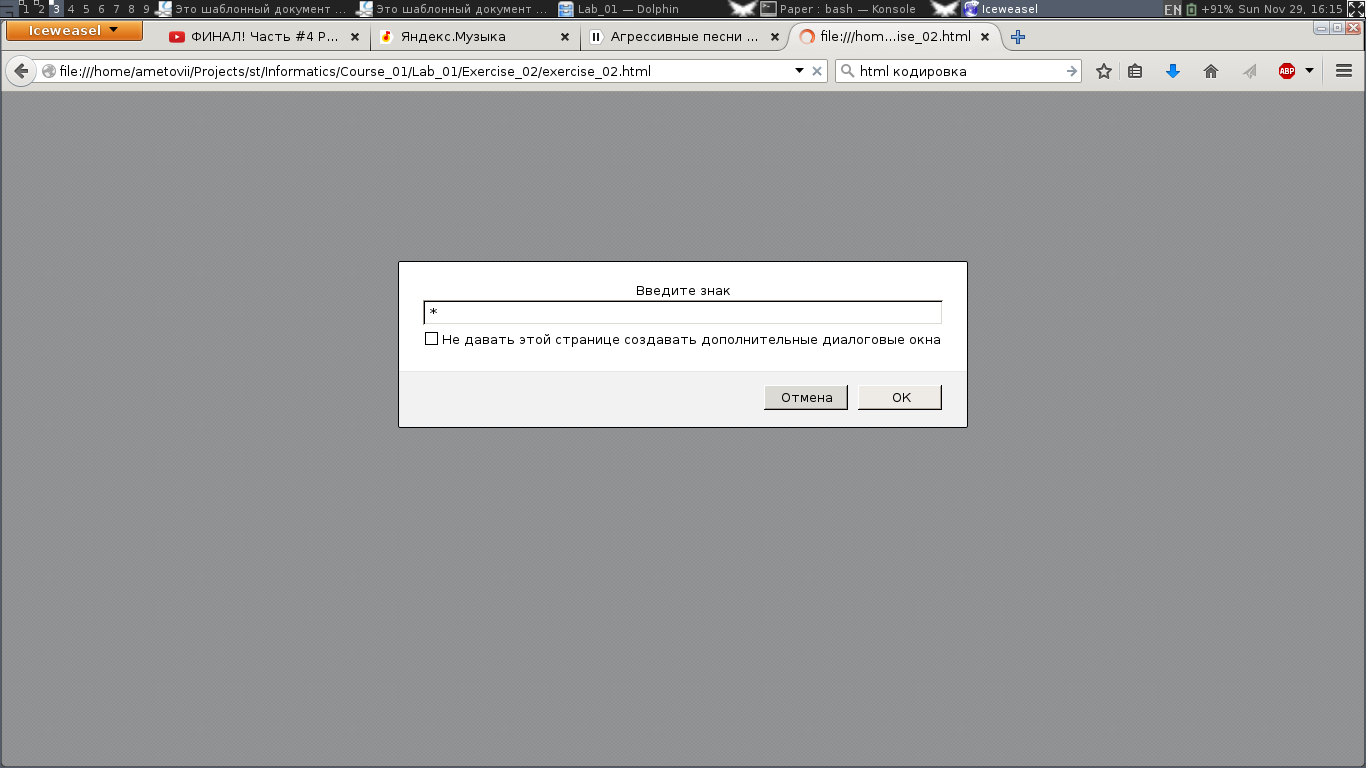
\includegraphics[width=15cm]{img/0207.png}
  
\includegraphics[width=15cm]{img/0208.png}
  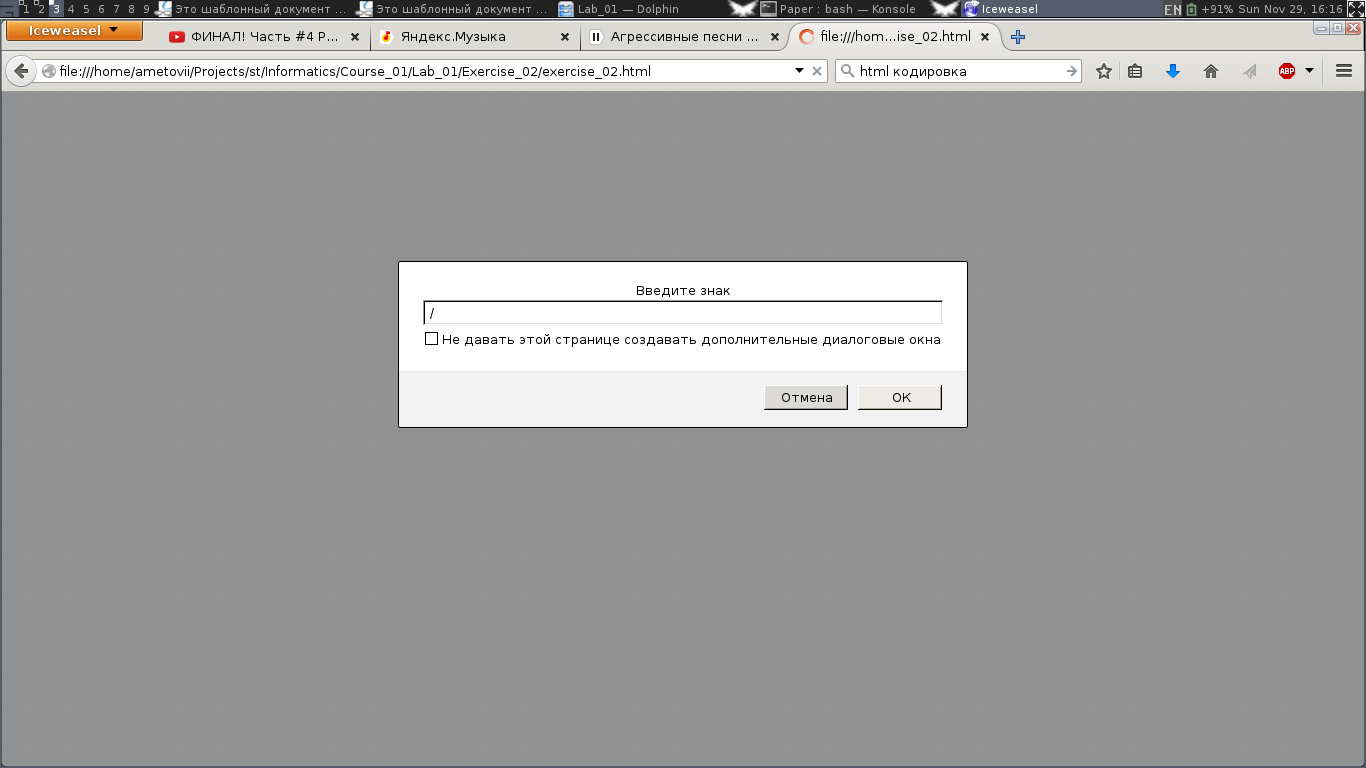
\includegraphics[width=15cm]{img/0209.png}
  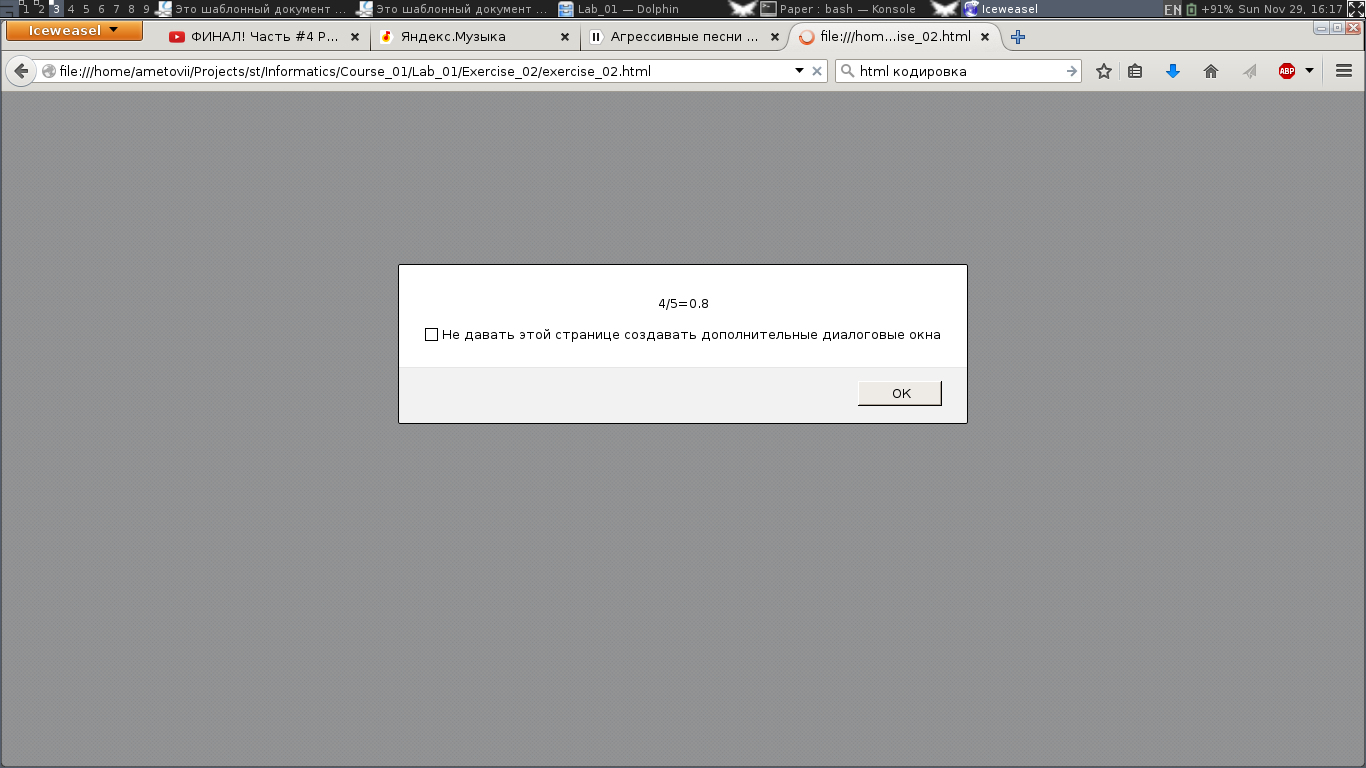
\includegraphics[width=15cm]{img/0210.png}
  
\includegraphics[width=15cm]{img/0211.png}
\end{center}

Исходный код \verb|exercise_02.html|:
\begin{verbatim}
<body>
  <head>
    <meta charset = "utf-8">
  </head>
  <script>
    a = parseInt (prompt ("Введите первое число"))
    b = parseInt (prompt ("Введите второе число"))
    operation = prompt ("Введите знак")
    if (operation == "*") alert (a + operation + b + "="
    + (a * b))
    if (operation == "+") alert (a + operation + b + "="
    + (a + b))
    if (operation == "-") alert (a + operation + b + "="
    + (a - b))
    if (operation == "/" && b != 0) alert (a + operation + b + "="
    + (a / b))
    if (operation == "/" && b == 0)
    alert ("Ошибка! На ноль делить нельзя.и")
  </script>
</body>
\end{verbatim}
